\documentclass[12pt, a4paper, oneside]{ctexart}
\usepackage{minted, multicol, geometry, graphicx, fancyvrb}
\usepackage{relsize, setspace, enumitem, float}

\geometry{a4paper, scale = 0.85}

\setenumerate[1]{itemsep=0pt,partopsep=0pt,parsep=\parskip,topsep=0pt}
\setitemize[1]{itemsep=0pt,partopsep=0pt,parsep=\parskip,topsep=0pt}
\setdescription{itemsep=0pt,pa
rtopsep=0pt,parsep=\parskip,topsep=0pt}
\setlength{\parindent}{0pt}

\setminted[cpp]{
	style=xcode,
	mathescape,
	linenos,
	autogobble,
	baselinestretch=1,
	tabsize=3,
	fontsize=\scriptsize,
	%bgcolor=Gray,
	frame=single,
	framesep=1mm,
	framerule=0.3pt,
	numbersep=1mm,
	breaklines=true,
	breaksymbolsepleft=2pt,
	%breaksymbolleft=\raisebox{0.8ex}{ \small\reflectbox{\carriagereturn}}, %not moe!
	%breaksymbolright=\small\carriagereturn,
	breakbytoken=false,
	% showtabs=true,
	% tab={\relscale{0.6} $\big\vert \ \ \ $ \relscale{1}},
}

\title{ACM 模板}
\author{钱智煊,黄佳瑞,车昕宇}
\date{\today}

\begin{document}
    \scriptsize
    \maketitle
    \newpage
    
    \begin{multicols}{2}
        \tableofcontents
        \newpage

        \section{图论}
        \subsection{连通性相关}
        \subsubsection{tarjan}
        \inputminted{cpp}{src/graph/tarjan.cpp}
        \subsubsection{tarjan求LCA}
        记录上一个访问的边时要记录边的编号,不能记录上一个过来的节点(因为会有重边)!!!

(如果选择在加边的时候特判,注意编号问题:用输入顺序来对应数组中位置的时候,重边跳过,但是需要 tot+=2。)

圆方树示意图:

\begin{figure}[H]
    \centering
    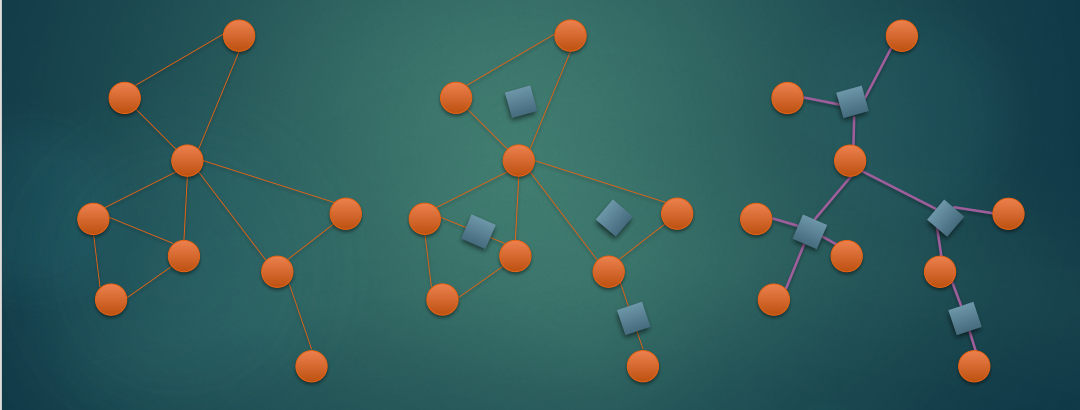
\includegraphics[width=0.45\textwidth]{src/graph/tarjan-tree.png}
    \caption{圆方树示意图}
\end{figure}

\inputminted{cpp}{src/graph/tarjan.cpp}
        \inputminted{cpp}{src/graph/tarjan_lca.cpp}
        \subsubsection{割点、割边}
        注意这里的 $dfn$ 表示\textbf{不经过父亲},能到达的最小的 $dfn$ 。
割点:
\begin{itemize}
    \item 若 $u$ 是根节点,当至少存在 $2$ 条边满足 $low(v)\ge dfn(u)$ 则 $u$ 是割点 。
    \item 若 $u$ 不是根节点,当至少存在 $1$ 条边满足 $low(v)\ge dfn(u)$ 则 $u$ 是割点 。
\end{itemize}
割边:
\begin{itemize}
    \item 当存在一条边条边满足 $low(v)>dfn(u)$ 则边 $i$ 是割边。
\end{itemize}
注意:
记录上一个访问的边时要记录边的编号,不能记录上一个过来的节点(因为会有重边)!!!或者在加边的时候特判一下,不过注意编号问题。(用输入顺序来对应数组中位置的时候,重边跳过,但是需要 tot+=2)
        \subsubsection{圆方树}
        \begin{figure}[H]
    \centering
    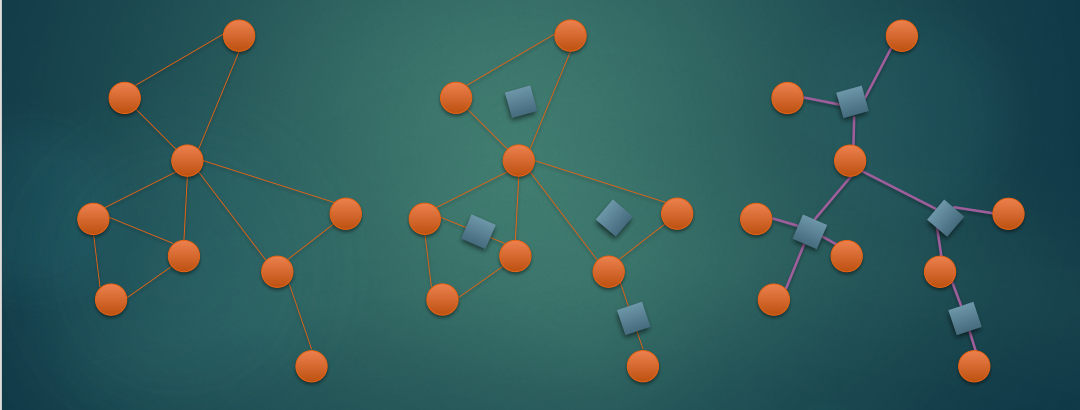
\includegraphics[width=\columnwidth]{src/graph/圆方树.png}
\end{figure}
圆方树会建立很多新的点,所以不要忘记\textbf{给数组开两倍}!
        \inputminted{cpp}{src/graph/圆方树.cpp}
        \subsection{同余最短路}
        形如:
\begin{itemize}
    \item 设问 $1$ :给定 $n$ 个整数,求这 $n$ 个整数在 $h(h\le2^{63}-1)$ 范围内 \textbf{能拼凑出多少的其他整数(整数可以重复取)} 。
    \item 设问 $2$ :给定 $n$ 个整数,求这 $n$ 个整数 \textbf{不能拼凑出的最小(最大)的整数} 。
\end{itemize}

设 $x$ 为 $n$ 个数中最小的一个,令 $ds[i]$ 为只通过增加其他 $n-1$ 种数能够达到的最低楼层 $p$ ,并且满足 $p\equiv i\pmod{x}$ 。

对于 $n-1$ 个数与 $x$ 个 $ds[i]$ ,可以如下连边:

\begin{minted}{cpp}
for(int i=0;i<x;i++) for(int j=2;j<=n;j++) add(i,(i+a[j])%x,a[j]);
\end{minted}

之后进行最短路 ,对于 :
\begin{itemize}
    \item 问在 $h$ 范围内能够到达的\textbf{点的数量}:答案为(加一因为 $i$ 本身也要计算)
    \[
    \sum_{i=0}^{x-1}{[d[i]\le h]\times\dfrac{h-d[i]}{x}+1}
    \]
    \item 问不能达到的\textbf{最小的数}:答案为:( $i$ 一定时最小表示的数为 $d[i]=s\times x+i$ ,则 $(s-1)\times x+i$  \textbf{一定不能} 被表示出来 )
    \[
    \min_{i=1}^{x-1}{\{d[i]-x\}}
    \]
\end{itemize}

\textbf{注意:$ds$ 与 $h$ 范围相同,一般也要开 $\operatorname{long}~\operatorname{long}$ !}

        \section{数据结构}
        \subsection{动态树}
        \inputminted{cpp}{src/data structure/LCT.cpp}

        \section{字符串}
        \subsection{后缀数组(与后缀树)}
        \inputminted{cpp}{src/string/SA.cpp}
        \subsection{AC自动机}
        \inputminted{cpp}{src/string/ACAM.cpp}
        \subsection{回文自动机}
        \inputminted{cpp}{src/string/PAM.cpp}
        \subsection{Manacher算法}
        \inputminted{cpp}{src/string/manacher.cpp}
        \subsection{KMP算法与border理论}
        \inputminted{cpp}{src/string/kmp.cpp}
字符串的border理论:
以下记字符串 $S$ 的长度为 $n$ 。
\begin{itemize}
    \item 若串 $S$ 具备长度为 $m$ 的 border ,则其必然具备长度为 $n-m$ 的周期,反之亦然。
    \item 弱周期性引理:若串 $S$ 存在周期 $p$ 、$q$ ,且 $p+q\le n$ ,则 $S$ 必然存在周期 $\gcd(p,q)$ 。
    \item 引理1:若串 $S$ 存在长度为 $m$ 的 border $T$,且 $T$ 具备周期 $p$ ,满足 $2m-n\ge p$ ,则 $S$ 同样具备周期 $p$ 。
    \item 周期性引理:若串 $S$ 存在周期 $p$ 、$q$ ,满足 $p+q-\gcd(p,q)\le n$ ,则串 $S$ 必然存在周期 $\gcd(p,q)$ 。
    \item 引理2:串 $S$ 的所有 border 的长度构成了 $O(\log n)$ 个不交的等差数列。更具体的,记串 $S$ 的最小周期为 $p$ ,则其所有长度包含于区间 $[n \bmod p + p, n)$ 的 border 构成了一个等差数列。
    \item 引理3:若存在串 $S$ 、$T$ ,使得 $2|T|\ge n$ ,则 $T$ 在 $S$ 中的所有匹配位置构成了一个等差数列。
    \item 引理4:PAM 的失配链可以被划分为 $O(\log n)$ 个等差数列。
\end{itemize}
        \subsection{Z函数}
        Z函数用于求解字符串的每一个后缀与其本身的 lcp 。其思路和 manacher 算法基本一致,都是维护一个扩展过的最右端点和对应的起点,而当前点要么暴力扩展使最右端点右移,要么处在记录的起点和终点间,从而可以利用已有的信息快速转移。
\inputminted{cpp}{src/string/zfunc.cpp}
    \end{multicols}
\end{document}
